\section{Floating Bubbles vs.\ Multi-Exchange Local Search: Why \texorpdfstring{$5\times 5$}{5x5} Is Harder Than \texorpdfstring{$10\times 10$}{10x10}}
\label{sec:bubble}

When we first encountered the discrete combination-lock traps of \Cref{sec:landscape} in \texttt{physics-lab.html}, a natural physical intuition suggested itself: what if the $n^2$ tiles were not locked into rigid grid squares at all, but could float continuously in two-dimensional space $\R^2$ like buoyant soap bubbles, sliding past one another to avoid discrete swap barriers? In the flagship application of our browser laboratory, the \emph{Bubble Trinity Simulator} (\texttt{bubble-trinity.html}, powered by \texttt{bubbleTrinityApp.js} \cite{mathewson2026physicalsolver}), we built both this continuous 2D bubble physics engine and a discrete multi-exchange local search engine (\emph{Auto Settler}) side by side. Watching the two engines compete on the same screen reveals two of the most instructive lessons of this project: why continuous 2D bubbles ``cheat'' by blending their heights between grid cells ($0.0\%$ discrete recovery even under exact Hungarian bipartite matching), and why discrete multi-exchange search solves $100.0\%$ of boards from $n=3$ to $n=10$ while finding $5\times 5$ harder than $10\times 10$.

\subsection{Why Continuous 2D Bubbles ``Cheat'': Spatial Amplitude Averaging vs.\ Permutation Saddles}

In \texttt{bubble-trinity.html}, the $n^2$ integers are represented as circular bubbles at continuous positions $\mathbf{r}_a(t) = (x_a(t), y_a(t)) \in \R^2$ ($a=1,\dots,n^2$) initialized at the grid centers $\mathbf{r}_a^{(0)} = (c_a - \frac{n+1}{2}, r_a - \frac{n+1}{2})$, with visual radii and buoyancy colors proportional to their heights $Z_a$. At each grid cell $b \in \{1,\dots,n^2\}$, a soft Gaussian kernel interpolates the nearby bubble heights to define an induced height vector $\widetilde{\mathbf{z}}(t)$ and continuous line energy $\Hind(t)$:
\begin{equation}
  W_{ab}(t) = \frac{\exp\bigl(-2\|\mathbf{r}_a(t) - \mathbf{r}_b^{(0)}\|_2^2\bigr)}{\sum_{a'=1}^{n^2} \exp\bigl(-2\|\mathbf{r}_{a'}(t) - \mathbf{r}_b^{(0)}\|_2^2\bigr)}, \qquad
  \widetilde{\mathbf{z}}(t) = W(t)^\top \mathbf{z}, \qquad
  \Hind(t) = \|A_n \widetilde{\mathbf{z}}(t)\|_2^2.
  \label{eq:kernel_induced_H}
\end{equation}
In the interactive Langevin loop of \texttt{bubbleTrinityApp.js}, each bubble moves with step size $\Delta t = 0.025$ and momentum persistence $\gamma_m \in [0,1)$ under the update
\begin{equation}
  \begin{aligned}
    \mathbf{v}_a(t+\Delta t) &= \gamma_m \mathbf{v}_a(t) + \Delta t\Bigl[\mathbf{F}_a^{\mathrm{well}} + \mathbf{F}_a^{\mathrm{cont}} + \mathbf{F}_a^{\mathrm{rep}} + \mathbf{F}_a^{\mathrm{field}} + \sigma_T \boldsymbol{\xi}_a(t)\Bigr], \\
    \mathbf{r}_a(t+\Delta t) &= \mathbf{r}_a(t) + \Delta t\,\mathbf{v}_a(t+\Delta t),
  \end{aligned}
  \label{eq:langevin_sde}
\end{equation}
which combines four user-adjustable sliders in the UI: lattice well springs $\mathbf{F}_a^{\mathrm{well}} = -k_w(\mathbf{r}_a - \mathbf{r}_a^{(0)})$ that pull bubbles toward home grid cells, radial dish containment $\mathbf{F}_a^{\mathrm{cont}} = -k_c \mathbf{r}_a$, bubble-to-bubble core repulsion $\mathbf{F}_a^{\mathrm{rep}} = c_r k_r \sum_{b\ne a} (\mathbf{r}_a - \mathbf{r}_b)/(\|\mathbf{r}_a - \mathbf{r}_b\|^2 + \epsilon_0)^{3/2}$ ($c_r=0.08, \epsilon_0=0.15$), and the magic-field drift $\mathbf{F}_a^{\mathrm{field}} = (c_f k_f + c_s k_s)(\mathbf{r}_a^{\mathrm{target}} - \mathbf{r}_a)$ ($c_f=0.25, c_s=0.65$) toward the stress-weighted centroid $\mathbf{r}_a^{\mathrm{target}}(t) = \sum_{b=1}^{n^2} \sigma_{ab}(t)\mathbf{r}_b^{(0)}$ with $\sigma_{ab}(t) \propto \exp(-Z_a (A_n^\top A_n\widetilde{\mathbf{z}}(t))_b / 250)$, plus thermal agitation $\boldsymbol{\xi}_a(t) \sim \mathcal{N}(\mathbf{0}, I_2)$ scaled by $\sigma_T = 0.12\,T$.

\begin{figure}[t]
  \centering
  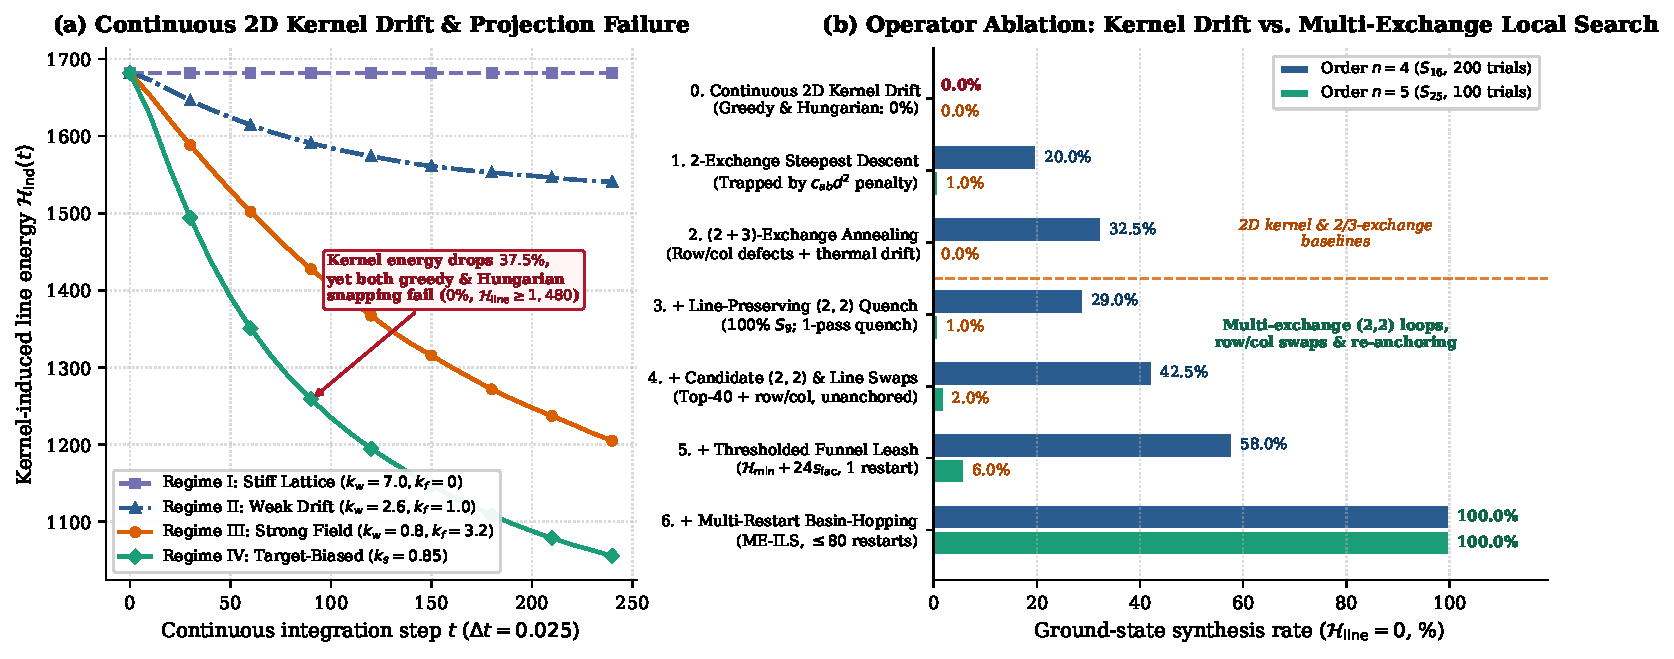
\includegraphics[width=\textwidth]{figures/fig6_bubble_trinity_regimes.pdf}
  \caption{\textbf{Continuous 2D Bubble Trinity trajectories and discrete local-search mechanism ablation.} \textbf{(a)} Trajectories of the kernel-induced line energy $\Hind(t)$ across $250$ integration steps ($\Delta t = 0.025$) for the four interactive presets of \Cref{tab:bubble_regimes}, starting from a $4$-swap perturbation of D\"urer's $4\times 4$ square ($\Hind(0) = 1{,}681.89$). Although continuous bubble drift reduces $\Hind(t)$ by $37.5\%$, both greedy snapping and exact Hungarian projection fail ($0\%$, $\Hline \ge 1{,}480$) because $\Hind(t)$ relaxes via convex amplitude averaging rather than discrete permutation swaps. \textbf{(b)} Operator ablation study (\Cref{tab:physical_analogs_ablation}) contrasting continuous 2D bubble drift and $2$/$3$-exchange heuristics (Tiers~$0\text{--}2$) against line-preserving $(2,2)$ plaquette moves, candidate-list $(2,2)$ swaps with row/column permutations, thresholded funnel re-anchoring, and multi-restart iterated local search (Tiers~$3\text{--}6$) at orders $n=4$ ($200$ trials) and $n=5$ ($100$ trials).}
  \label{fig:bubble_trinity}
\end{figure}

\begin{table}[t]
\centering
\caption{Slider parameters and trajectory invariants across the four interactive presets of \texttt{bubble-trinity.html} at order $n=4$ ($250$ steps, $\Delta t=0.025$), verified by \texttt{verify\_paper\_d.py}.}
\label{tab:bubble_regimes}
\resizebox{\textwidth}{!}{%
\begin{tabular}{@{}lccccccc@{}}
\toprule
Bubble Trinity Preset & $(k_f, k_r, k_w, k_c)$ & $(\gamma_m, k_s, T)$ & $\Hind(0)$ & $\Hind(250)$ & Min $\Hind$ & Mean $\Delta r_{\mathrm{rms}}$ & Max $\Delta r_{\mathrm{rms}}$ \\
\midrule
I. Frozen Lattice      & $(0.0, 0.0, 7.0, 0.0)$ & $(0.94, 0.00, 0.0)$ & $1681.89$ & $1681.89$ & $1681.89$ & $0.0000$ & $0.0000$ \\
II. Slow Drift         & $(1.0, 0.4, 2.6, 0.0)$ & $(0.82, 0.00, 0.5)$ & $1681.89$ & $1539.22$ & $1539.22$ & $0.0774$ & $0.1134$ \\
III. Field Storm       & $(3.2, 1.0, 0.8, 0.4)$ & $(0.60, 0.00, 1.2)$ & $1681.89$ & $1194.88$ & $1194.88$ & $0.2654$ & $0.4646$ \\
IV. Centrifugal Balance& $(2.2, 0.5, 1.8, 0.5)$ & $(0.75, 0.85, 0.4)$ & $1681.89$ & $1050.55$ & $1050.55$ & $0.4281$ & $0.6381$ \\
\bottomrule
\end{tabular}%
}
\end{table}

\Cref{fig:bubble_trinity}a and \Cref{tab:bubble_regimes} trace the continuous energy $\Hind(t)$ across the four named presets of \texttt{bubble-trinity.html}, starting from a $4$-swap perturbation of D\"urer's $4\times 4$ square ($\Hind(0) = 1{,}681.89$, discrete $\Hline = 2{,}336$). As the user switches from \emph{I.~Frozen Lattice} ($\Delta r_{\mathrm{rms}} = 0.0000$) and \emph{II.~Slow Drift} ($\langle\Delta r_{\mathrm{rms}}\rangle = 0.0774$) to \emph{III.~Field Storm} ($\max\Delta r_{\mathrm{rms}} = 0.4646$) and \emph{IV.~Centrifugal Balance} ($\max\Delta r_{\mathrm{rms}} = 0.6381$), the bubbles swirl across cell borders and the continuous energy gauge $\Hind(t)$ drops by $37.5\%$ to $1{,}050.55$. Yet the moment the user clicks ``Snap to Grid'' to project the floating bubbles $\{\mathbf{r}_a(t)\}$ back onto a discrete permutation $S \in S_{16}$, the magic square fails to materialize ($0.0\%$ recovery across all four presets, Tier~$0$ in \Cref{fig:bubble_trinity}b). Even when we replace greedy nearest-cell snapping ($\min_t \Hline(S_{\mathrm{greedy}}) = 1{,}480$) with exact $O(N^3)$ Hungarian / Kuhn--Munkres minimum-weight bipartite matching $\min_{\pi\in S_{n^2}}\sum_a \|\mathbf{r}_a(t) - \mathbf{r}_{\pi(a)}^{(0)}\|_2^2$ at every time step, the discrete energy never improves beyond its starting value ($\min_t \Hline(S_{\mathrm{Hung}}) = 2{,}336$, $0.0\%$ convergence). The reason is both visually obvious in the browser and mathematically fundamental: because the Gaussian weight matrix $W(t)$ in \Cref{eq:kernel_induced_H} is only column-stochastic rather than doubly stochastic and $\Hind(t)$ is convex in $\widetilde{\mathbf{z}}$, the bubbles ``cheat'' by parking on the boundary lines between grid cells so that positive and negative heights $Z_a$ blend together toward zero in the interior of the assignment polytope, rather than executing the discrete multi-tile exchanges required to cross permutation saddles.

\subsection{How the Discrete Auto-Settler Unlocks the Board: Multi-Exchange Local Search}

If floating bubbles in $\R^2$ get stuck by blending their amplitudes, how does the discrete \emph{Auto Settler} button in \texttt{bubble-trinity.html} and \texttt{physics-lab.html} rapidly snap scrambled boards into exact magic squares? Note first that if one merely wants to write down a single magic square of order $n$, classical closed-form rules (Siamese, doubly-even mask, Conway LUX) do so in $O(n^2)$ steps, and specialized constraint-based local search (CBLS) / tabu solvers \cite{codognet2001yet,vanhentenryck2005constraint} reach $n \sim 100$ by restricting swaps to defective lines. Our goal in the interactive lab is different: we want to watch a physical energy landscape $\Hline(S)$ relax from arbitrary random permutations and understand \emph{which collective multi-tile moves unlock its traps}. \Cref{tab:physical_analogs_ablation} and \Cref{fig:bubble_trinity}b report a controlled ablation study across six relaxation tiers at orders $n=4$ ($200$ random starts) and $n=5$ ($100$ random starts).

As shown in \Cref{rem:low_mode_insufficiency} and Section~5.1, macroscopic tilt balance (blind to the $2n-4$ higher-degree polynomial moments) and continuous 2D bubble drift (Tier~$0$) both fail to reach $\Hline = 0$. On the discrete grid, pure $2$-exchange steepest descent (Tier~$1$, single-pair swaps \cite{kawasaki1966diffusion}) freezes whenever $-2d(g_a-g_b) + c_{ab}d^2 \ge 0$ for all pairs $(a,b)$, succeeding on $74.5\%$ of $S_9$, $20.0\%$ of $S_{16}$, and only $1.0\%$ of $S_{25}$. Adding $3$-exchange triplet rotations under a $1{,}500$-step simulated annealing schedule (Tier~$2$, \cite{kirkpatrick1983optimization}) fails to unlock the order-$3$ trap $S_{\mathrm{trap}}^{(3)}$ ($0/8$ escapes) and achieves only $32.5\%$ at $n=4$ and $0.0\%$ at $n=5$, because $3$-cycles cannot swap elements between two columns while preserving their row sums, and unanchored thermal random walks wander out of narrow low-energy funnels.

Our \emph{Multi-Exchange Iterated Local Search (ME-ILS)} engine overcomes these bottlenecks step by step across Tiers~$3\text{--}6$. First, augmenting $2$-exchange descent with the $2\binom{n}{2}^3$ row- and column-preserving $(2,2)$ plaquette moves (Tier~$3$---synchronized $4$-tile combination moves bounded by a single-swap saddle filter $\Delta\Hline(\tau_1) \le 80 s_{\mathrm{fac}}(n)$ where $s_{\mathrm{fac}}(n) = \max(1, \lfloor(n/4)^2\rfloor)$) unlocks $100.0\%$ of $S_9$ and raises single-quench recovery on $S_{16}$ from $20.0\%$ to $29.0\%$. Second, expanding the local escape neighborhood at $2$-exchange minima to include whole-row and whole-column swaps ($2\binom{n}{2}$ zero-barrier moves that preserve all row and column sums while shearing the two main diagonals) together with disjoint pairs selected from the top $K=40$ single swaps with $\Delta\Hline(\tau_1) \le 48 s_{\mathrm{fac}}(n)$ (Tier~$4$, with $5$ unanchored basin kicks in a single restart) raises $n=4$ convergence to $42.5\%$. Third, adding a threshold-bounded re-anchoring leash (Tier~$5$, which remembers the deepest local minimum $S_{\min}$ found within a restart and snaps back to $S_{\min}$ whenever a $2$-swap kick followed by steepest descent exceeds $\Hline(S_{\min}) + 24 s_{\mathrm{fac}}(n)$ across $18$ kicks) keeps the solver tethered to the bottom of the funnel and raises single-restart $n=4$ convergence to $58.0\%$. Finally, wrapping this tethered funnel search in an outer multi-restart basin-hopping loop ($\le 80$ restarts, Tier~$6$ \cite{wales1997global,wales2003energy}) achieves $100.0\%$ ground-state convergence across all orders $n = 3, 4, 5, 6, 7, 8, 9, 10$.

\begin{table}[t]
\centering
\caption{Controlled ablation study contrasting continuous 2D bubble drift and $2$/$3$-exchange heuristics (Tiers~$0\text{--}2$) against cooperative $(2,2)$ plaquette moves, row/column permutations, thresholded funnel re-anchoring, and multi-restart basin-hopping (Tiers~$3\text{--}6$), certified by \texttt{verify\_paper\_d.py}.}
\label{tab:physical_analogs_ablation}
\resizebox{\textwidth}{!}{%
\begin{tabular}{@{}llllccc@{}}
\toprule
\textbf{Tier} & \textbf{Relaxation / Local-Search Mechanism} & \textbf{Move Neighborhood} & \textbf{Primary Bottleneck or Escape Mechanism} & \textbf{$n=3$ ($S_9$)} & \textbf{$n=4$ ($S_{16}$)} & \textbf{$n=5$ ($S_{25}$)} \\
\midrule
\textbf{--} & Linear Dipole \& Diagonal Balance & $4$ global linear modes & Blind to $2n-4$ higher-degree polynomial moments (\Cref{rem:low_mode_insufficiency}: $S_{\mathrm{low}}$, $\Hline=1{,}584$) & Fails & Fails & Fails \\
\textbf{0} & Continuous 2D Bubble Drift + Snap & Greedy \& Hungarian snap & Bubbles blend heights across cell borders ($\min\Hline \ge 1{,}480$) & $0.0\%$ & $0.0\%$ & $0.0\%$ \\
\textbf{1} & $2$-Exchange Steepest Descent \cite{kawasaki1966diffusion} & $\binom{n^2}{2}$ pair swaps & Traps when quadratic recoil $c_{ab}d^2 \ge 8$ blocks $-2d(g_a-g_b)$ (\Cref{lem:swap_law}) & $74.5\%$ & $20.0\%$ & $1.0\%$ \\
\textbf{2} & $(2+3)$-Exchange Simulated Annealing \cite{kirkpatrick1983optimization} & $2$- \& $3$-cycles ($B=1{,}500$) & $3$-cycles break row/col conservation ($0/8$ on $S_{\mathrm{trap}}^{(3)}$); thermal walk loses funnel & $74.5\%$ & $32.5\%$ & $0.0\%$ \\
\midrule
\textbf{3} & $+$ Line-Preserving $(2,2)$ Plaquette Quench & $2\binom{n}{2}^3$ row/col $(2,2)$ loops & Preserves row/col sums while cancelling conjugate column/row dipoles ($1$ quench) & $\mathbf{100.0\%}$ & $29.0\%$ & $1.0\%$ \\
\textbf{4} & $+$ Candidate $(2,2)$ \& Row/Col Permutations & Top-$40$ $(2,2)$ + $2\binom{n}{2}$ lines & Zero-barrier row/col swaps shear diagonals ($5$ unanchored kicks, $1$ restart) & $\mathbf{100.0\%}$ & $42.5\%$ & $2.0\%$ \\
\textbf{5} & $+$ Thresholded Funnel Re-Anchoring & Leash $\Hline \le \mathcal{H}_{\min}+24s_{\mathrm{fac}}$ & Snaps back to deepest minimum $S_{\min}$ on high kicks ($18$ kicks, $1$ restart) & $\mathbf{100.0\%}$ & $58.0\%$ & $6.0\%$ \\
\textbf{6} & $+$ Multi-Restart Basin-Hopping (ME-ILS) \cite{wales1997global} & $\le 80$ re-anchored restarts & Iterated local search across independent funnel basins ($18$ kicks/restart) & $\mathbf{100.0\%}$ & $\mathbf{100.0\%}$ & $\mathbf{100.0\%}$ \\
\bottomrule
\end{tabular}%
}
\end{table}

\begin{table}[t]
\centering
\caption{Multi-order synthesis benchmark of Multi-Exchange Iterated Local Search (ME-ILS) across orders $n = 3, 4, 5, 6, 7, 8, 9, 10$ with order-scaled thresholds $s_{\mathrm{fac}}(n) = \max(1,\lfloor(n/4)^2\rfloor)$, certified by \texttt{verify\_paper\_d.py}. We report the nullspace-to-constraint ratio $\eta_{\mathrm{MC}}(n) = (n^2-2n-1)/(2n)$, the fraction $f_{\mathrm{null}}(n) = 1 - 2/(n-1)^2$ of the semi-magic $(2,2)$ subspace $\mathcal{V}_{\mathrm{row}}\otimes\mathcal{V}_{\mathrm{col}}$ orthogonal to both diagonals, and the per-step $2$-cycle pair neighborhood $\binom{n^2}{2}$.}
\label{tab:multi_order_settler}
\resizebox{\textwidth}{!}{%
\begin{tabular}{@{}ccccccccccc@{}}
\toprule
Order $n$ & State Space $n^2!$ & Nullity $\dim\ker(\Ltilde_n)$ & Ratio $\eta_{\mathrm{MC}}$ & Diag-Free $(2,2)$ $f_{\mathrm{null}}$ & Pairs $\binom{n^2}{2}$ & Success ($\Hline=0$) & Mean Descents & Mean Pair Evals & Mean Restarts & Mean Time \\
\midrule
$n=3$  & $9! = 3.63\times 10^5$      & $2$  & $0.33$ & $50.0\%$ & $36$    & $\mathbf{200 / 200}$ ($\mathbf{100.0\%}$) & $5.1$   & $184$       & $0.00$ & $0.1\text{ ms}$ \\
$n=4$  & $16! = 2.09\times 10^{13}$  & $7$  & $0.88$ & $77.8\%$ & $120$   & $\mathbf{200 / 200}$ ($\mathbf{100.0\%}$) & $52.9$  & $6{,}348$     & $0.70$ & $4.9\text{ ms}$ \\
$n=5$  & $25! = 1.55\times 10^{25}$  & $14$ & $1.40$ & $87.5\%$ & $300$   & $\mathbf{100 / 100}$ ($\mathbf{100.0\%}$) & $466.6$ & $139{,}980$   & $8.03$ & $108.9\text{ ms}$ \\
$n=6$  & $36! = 3.72\times 10^{41}$  & $23$ & $1.92$ & $92.0\%$ & $630$   & $\mathbf{100 / 100}$ ($\mathbf{100.0\%}$) & $446.8$ & $281{,}484$   & $7.28$ & $208.8\text{ ms}$ \\
$n=7$  & $49! = 6.08\times 10^{62}$  & $34$ & $2.43$ & $94.4\%$ & $1{,}176$ & $\mathbf{100 / 100}$ ($\mathbf{100.0\%}$) & $267.5$ & $314{,}580$   & $4.02$ & $218.0\text{ ms}$ \\
$n=8$  & $64! = 1.27\times 10^{89}$  & $47$ & $2.94$ & $95.9\%$ & $2{,}016$ & $\mathbf{100 / 100}$ ($\mathbf{100.0\%}$) & $294.5$ & $593{,}712$   & $4.32$ & $407.0\text{ ms}$ \\
$n=9$  & $81! = 5.80\times 10^{120}$ & $62$ & $3.44$ & $96.9\%$ & $3{,}240$ & $\mathbf{50 / 50}$ ($\mathbf{100.0\%}$)   & $293.0$ & $949{,}320$   & $4.06$ & $658.1\text{ ms}$ \\
$n=10$ & $100! = 9.33\times 10^{157}$& $79$ & $3.95$ & $97.5\%$ & $4{,}950$ & $\mathbf{50 / 50}$ ($\mathbf{100.0\%}$)   & $258.5$ & $1{,}279{,}575$ & $3.34$ & $880.8\text{ ms}$ \\
\bottomrule
\end{tabular}%
}
\end{table}

\subsection{Why \texorpdfstring{$5\times 5$}{5x5} Requires More Restarts Than \texorpdfstring{$10\times 10$}{10x10}: Nullspace Dimensional Relief}

\Cref{tab:multi_order_settler} and \Cref{fig:dimensional_relief} summarize the performance of ME-ILS across all eight orders $n = 3, 4, 5, 6, 7, 8, 9, 10$ ($900 / 900$ total trials reaching $\Hline = 0$, spanning up to $100! \approx 9.33\times 10^{157}$ states at $n=10$). Looking across the rows of \Cref{tab:multi_order_settler}, a counterintuitive pattern jumps out: the number of basin-hopping restarts and descent loops required to find a magic square does \emph{not} grow monotonically with board size! Instead, search difficulty peaks sharply at order $n=5$ ($8.03$ mean restarts and $466.6$ descent loops) and then \emph{declines} across $n=6,7,8,9,10$, requiring only $3.34$ mean restarts and $258.5$ descent loops at $n=10$.

The spectral decomposition of \Cref{prop:spectral_rationalization} explains why larger boards become topologically easier to untangle even as their per-step pair evaluations $\binom{n^2}{2} = O(n^4)$ grow. Every row- or column-preserving $(2,2)$ plaquette move acts via a vector $(\mathbf{e}_{r_1}-\mathbf{e}_{r_2})\otimes(\mathbf{e}_{c_1}-\mathbf{e}_{c_2})$ inside the $(n-1)^2$-dimensional semi-magic subspace $\mathcal{V}_{\mathrm{row}}\otimes\mathcal{V}_{\mathrm{col}} = \ker(L_{\mathrm{rc}})$. Because the two main diagonals impose only $2$ linear constraints ($\widetilde{\mathbf{s}}_d, \mathbf{a}_d$) on $\mathcal{V}_{\mathrm{row}}\otimes\mathcal{V}_{\mathrm{col}}$, the fraction of the $(2,2)$ plaquette subspace that lies inside the exact magic nullspace $\ker(\Ltilde_n)$ is
\begin{equation}
  f_{\mathrm{null}}(n) = \frac{\dim\ker(\Ltilde_n)}{\dim(\mathcal{V}_{\mathrm{row}}\otimes\mathcal{V}_{\mathrm{col}})} = \frac{n^2 - 2n - 1}{(n-1)^2} = 1 - \frac{2}{(n-1)^2},
  \label{eq:null_plaquette_fraction}
\end{equation}
alongside the Maxwell--Calladine nullspace-to-constraint ratio $\eta_{\mathrm{MC}}(n) = (n^2-2n-1)/(2n)$ (\Cref{eq:maxwell_calladine_ratio}). At $n=3$ and $n=4$, the state spaces are small enough that $(2,2)$ moves and one or two restarts immediately find a ground state; at $n=5$ ($\eta_{\mathrm{MC}} = 1.40$, $f_{\mathrm{null}} = 87.5\%$), the state space is already huge ($25! \approx 1.55\times 10^{25}$) while the diagonal constraints still block $12.5\%$ of the semi-magic subspace, creating maximal frustration ($8.03$ restarts). For $n \ge 6$, however, $f_{\mathrm{null}}(n)$ climbs from $92.0\%$ ($n=6$) to $97.5\%$ ($n=10$), meaning that almost every row/column-preserving $(2,2)$ move is automatically invisible to the diagonals! With order-scaled energy thresholds $s_{\mathrm{fac}}(n) = \max(1,\lfloor(n/4)^2\rfloor)$, mean restarts drop to $7.28$ ($n=6$), $4.02$ ($n=7$), $4.32$ ($n=8$), $4.06$ ($n=9$), and $3.34$ ($n=10$), while total wall-clock time scales smoothly with the $\binom{n^2}{2}$ pair neighborhood ($880.8\text{ ms}$ at $n=10$).

\begin{figure}[t]
  \centering
  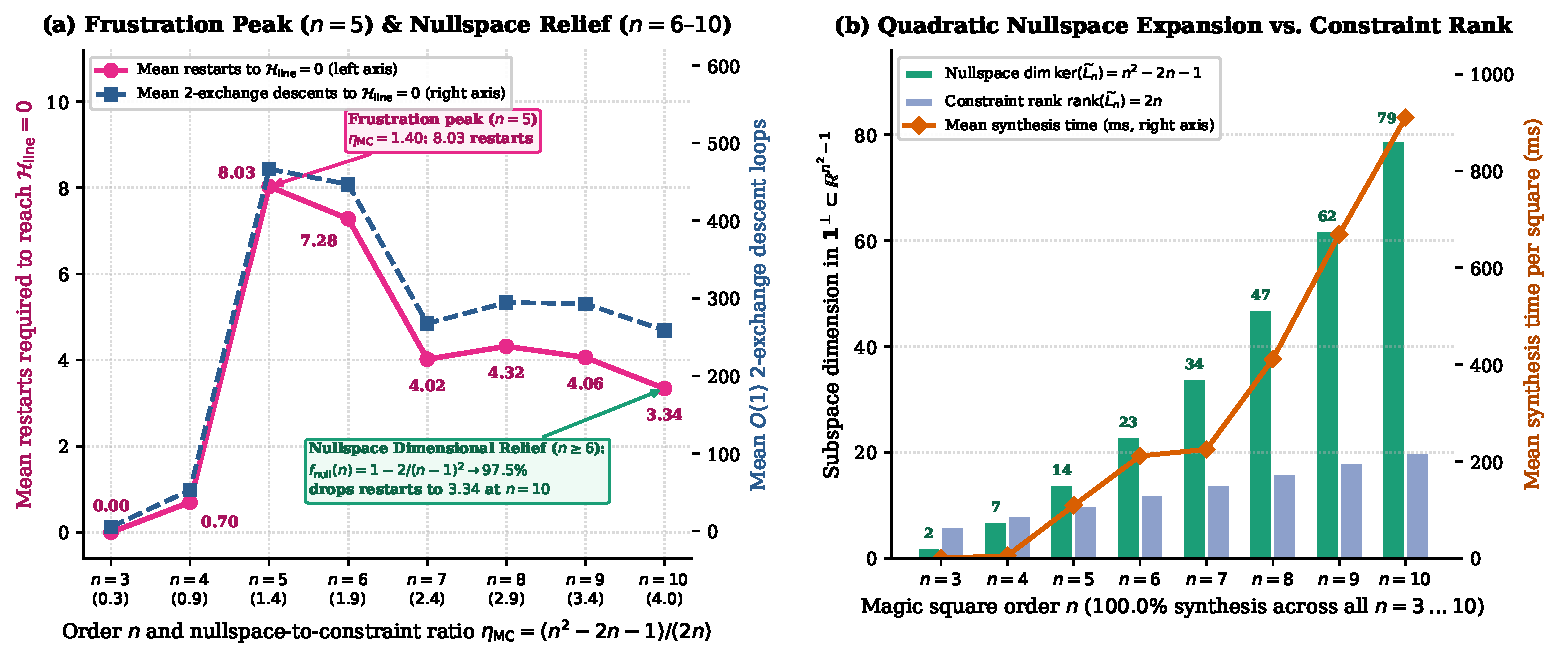
\includegraphics[width=\textwidth]{figures/fig7_multi_order_dimensional_relief.pdf}
  \caption{\textbf{Multi-order $100\%$ ground-state synthesis ($n=3\dots 10$) and nullspace dimensional relief.} \textbf{(a)} Mean restarts (magenta, left axis) and mean $O(1)$ incremental $2$-cycle descent loops (blue dashed, right axis) required by Multi-Exchange Iterated Local Search (ME-ILS) to reach $\Hline = 0$ with $100.0\%$ success across orders $n=3\dots 10$ (\Cref{tab:multi_order_settler}). Combinatorial frustration peaks at $n=5$ ($\eta_{\mathrm{MC}} = 1.40$: $8.03$ restarts, $466.6$ descents) and declines across $n=6\dots 10$ ($3.34$ restarts and $258.5$ descents at $n=10$) as the diagonal-free $(2,2)$ subspace fraction $f_{\mathrm{null}}(n) = 1 - 2/(n-1)^2$ reaches $97.5\%$. \textbf{(b)} Quadratic expansion of the magic nullspace $\dim\ker(\Ltilde_n) = n^2-2n-1$ (green bars, labeled with $\eta_{\mathrm{MC}}$) versus linear growth of the constraint rank $\operatorname{rank}(\Ltilde_n)=2n$ (blue bars) and mean synthesis runtime per square (orange curve, right axis).}
  \label{fig:dimensional_relief}
\end{figure}
